\let\negmedspace\undefined
\let\negthickspace\undefined
\documentclass[journal]{IEEEtran}
\usepackage[a5paper, margin=10mm, onecolumn]{geometry}
%\usepackage{lmodern} % Ensure lmodern is loaded for pdflatex
\usepackage{tfrupee} % Include tfrupee package

\setlength{\headheight}{1cm} % Set the height of the header box
\setlength{\headsep}{0mm}     % Set the distance between the header box and the top of the text

\usepackage{gvv-book}
\usepackage{gvv}
\usepackage{cite}
\usepackage{amsmath,amssymb,amsfonts,amsthm}
\usepackage{algorithmic}
\usepackage{graphicx}
\usepackage{textcomp}
\usepackage{xcolor}
\usepackage{txfonts}
\usepackage{listings}
\usepackage{enumitem}
\usepackage{mathtools}
\usepackage{gensymb}
\usepackage{comment}
\usepackage[breaklinks=true]{hyperref}
\usepackage{tkz-euclide} 
\usepackage{listings}
% \usepackage{gvv}                                        
\def\inputGnumericTable{}                                 
\usepackage[latin1]{inputenc}                                
\usepackage{color}                                            
\usepackage{array}                                            
\usepackage{longtable}                                       
\usepackage{calc}                                             
\usepackage{multirow}                                         
\usepackage{hhline}                                           
\usepackage{ifthen}                                           
\usepackage{lscape}
\begin{document}

\bibliographystyle{IEEEtran}
\vspace{3cm}

\title{Ellipse Question}
\author{EE24BTECH11040 - Mandara Hosur}
% \maketitle
% \newpage
% \bigskip
{\let\newpage\relax\maketitle}

\renewcommand{\thefigure}{\theenumi}
\renewcommand{\thetable}{\theenumi}
\setlength{\intextsep}{10pt} % Space between text and floats


\numberwithin{equation}{enumi}
\numberwithin{figure}{enumi}
\renewcommand{\thetable}{\theenumi}

\textbf{Question:}\\
Given that the length of the major axis of a conic is 16 units and the coordinates of the foci are $\brak{0,\pm6}$, find the equation of the conic.
\\ \\
\textbf{Solution:} \\
\begin{table}[h!]
  \centering
  \begin{tabular}[12pt]{ |c| c| c|}
    \hline
    \textbf{Variable} & \textbf{Description} & \textbf{Value}\\ 
    \hline
    $2k$ & Length of major axis & $16$ \\
    \hline 
    $\vec{F_1}$ & One of the foci of the conic & $\myvec{0\\6}$\\
    \hline
    $\vec{F_2}$ & Other foci of the conic & $\myvec{0\\-6}$\\
    \hline
\end{tabular}

  \caption{Given Information}
  \label{Table 1}
\end{table} \\
2 foci exist for this conic. Therefore, it must be an ellipse or a hyperbola.
\\
The general equation of a conic with directrix $\vec{n}^\top\vec{x}=c$ can be written as 
\begin{align}
g(\vec{x}) = \vec{x}^\top\vec{V}\vec{x}+2\vec{u}^\top\vec{x}+f \label{eq1}
\end{align}
\\
\begin{align}
\vec{u} =\frac{\vec{F_1}+\vec{F_2}}{2}=\myvec{0\\0} \text{ and } \vec{n}\equiv\vec{F_1}-\vec{F_2}\equiv\myvec{0\\1} \label{eq2}
\end{align}
\\
From \eqref{eq2}, we can conclude that we have a standard conic, with its center at the origin, foci on a coordinate axis (y-axis), and directrices parallel to a coordinate axis (x-axis).
\\
Therefore conic equation is either 
\begin{align}
\frac{x^2}{a^2} + \frac{y^2}{b^2} = 1 \text{ or } \frac{x^2}{a^2} - \frac{y^2}{b^2} = -1 \label{eq3}
\end{align}
\\
Given that $e \brak{=\sqrt{1\pm\frac{a^2}{b^2}}}$ represents the eccentricity of the conic, comparing \eqref{eq3} and \eqref{eq1} gives the relation
\begin{align}
\vec{V} = \myvec{1&0\\0&1-e^2}
\end{align}
\\
We know that the major axis is the y-axis. Assume some point $\myvec{0\\k}$ on the y-axis that satisfies \eqref{eq1}. This gives
\begin{align}
k = \sqrt{\frac{|f|}{|1-e^2|}}
\\
\implies 2k = 16 = 2\sqrt{\frac{|f|}{|1-e^2|}} \label{eq6}
\end{align}
\\
Rearranging \eqref{eq6} gives 
\begin{align}
8\sqrt{|1-e^2|}=\sqrt{|f|} \label{eq7}
\end{align}

Now, $\vec{F}=\frac{ce^2\vec{n}-\vec{u}}{\lambda_2}$ and $\lambda_2=\norm{n}^2$.
\\
\begin{align}
\implies\vec{F}=\frac{ce^2\vec{n}-\vec{u}}{\norm{n}^2} \label{eq8}
\end{align}
Substituting values of $\vec{F_1}$, $\vec{F_2}$, $\vec{n}$, and $\vec{u}$ and simplifying reduces \eqref{eq8} to
\begin{align}
\pm ce^2=6 \label{eq9}
\end{align}

Consider another equation $$c=\frac{e\vec{u}^\top\vec{n}\pm\sqrt{e^2\brak{\vec{u}^\top\vec{n}}^2-\lambda_2\brak{e^2-1}\brak{\norm{\vec{u}}^2-\lambda_2f}}}{\lambda_2e\brak{e^2-1}}$$
Substituting known values gives
\begin{align}
c=\pm\frac{1}{e}\sqrt{\frac{|f|}{|e^2-1|}} \label{eq10}
\end{align}

We have 3 equations (\eqref{eq7}, \eqref{eq9}, \eqref{eq10}) and 3 variables ($c$, $f$, $e$).
\\ \\
Upon solving, we get $e=\frac{3}{4}$, $c=\pm\frac{32}{3}$, and $|f|=28$
\\
However, $f$ can only have one value (either $+28$ or $-28$).
\\
To find this, assume some point $\brak{0,\alpha}$ to lie on the major axis of the conic. Substituting this point in the general conic equation \eqref{eq1} along with values of $\vec{V}$ and $\vec{u}$ gives $$\frac{7\alpha^2}{16}+f=0$$
This implies that $f$ must be negative, and therefore $f=-28$.
\\ \\
The equation of the conic thus becomes $$g(\vec{x}) = \vec{x}^\top\myvec{1&0\\0&\frac{7}{16}}\vec{x}-28$$

\begin{figure}[h]
	\centering
	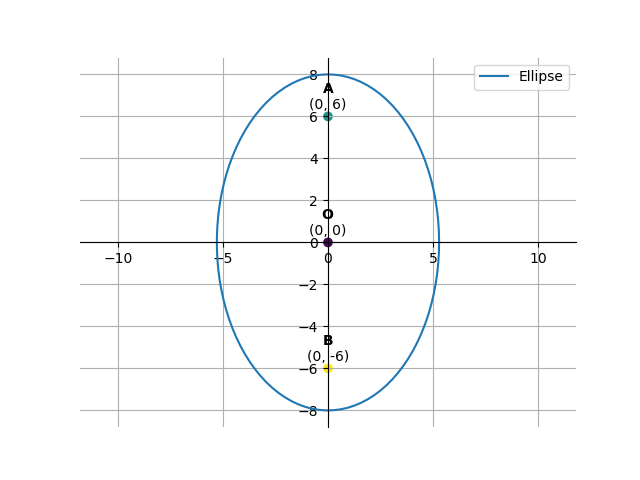
\includegraphics[width=\columnwidth]{figs/fig.png}
	\caption{Plot of conic}
\end{figure}

\end{document}
